%
% File acl2020.tex
%
%% Based on the style files for ACL 2020, which were
%% Based on the style files for ACL 2018, NAACL 2018/19, which were
%% Based on the style files for ACL-2015, with some improvements
%%  taken from the NAACL-2016 style
%% Based on the style files for ACL-2014, which were, in turn,
%% based on ACL-2013, ACL-2012, ACL-2011, ACL-2010, ACL-IJCNLP-2009,
%% EACL-2009, IJCNLP-2008...
%% Based on the style files for EACL 2006 by 
%%e.agirre@ehu.es or Sergi.Balari@uab.es
%% and that of ACL 08 by Joakim Nivre and Noah Smith

\documentclass[11pt,a4paper]{article}
\usepackage[hyperref]{acl2020}
\usepackage{times}
\usepackage{latexsym}
\usepackage{graphicx}
\usepackage{hyperref}
\renewcommand{\UrlFont}{\ttfamily\small}

\usepackage{microtype}

\aclfinalcopy % Uncomment this line for the final submission #TODO 
%\def\aclpaperid{***} %  Enter the acl Paper ID here


\newcommand\BibTeX{B\textsc{ib}\TeX}

\title{Multimodal Embeddings} 

\author{
  \textbf{Jan Kels} \\
  Heinrich Heine Universität \\
  Düsseldorf, Germany \\
  \texttt{Jan.Kels@hhu.de} \\ \\\And
  \textbf{Omar Hassan}\\
  Heinrich Heine Universität \\
  Düsseldorf, Germany \\
  \texttt{Omar.Hassan@hhu.de}
  }

\date{24.05.2023}  % won't actually show

\begin{document}
\maketitle

%\begin{abstract} %do we even need this part?
%  we present the concept of multimodal embedding and highlight the CLIP model architecture.
%\end{abstract}

\section{Introduction} %seem repetitive
Multimodal learning involves combining different channels of information to understand our environment. Humans possess five basic senses that enable us to perceive and comprehend the world. Similarly, AI researchers aim to train deep learning models that can effectively integrate different modalities. Two key challenges arise in multimodal learning. Firstly, there is a need to represent unstructured data numerically (embeddings or representations), this has been researched extensively in the last decade in two main modalities, text and image. Secondly, how to combine the representations of these different modalities effectively. \cite{akkus2023multimodal}

\section{Language Embeddings}
Representing language numerically has developed largely over the last decade. Starting with learning word embeddings which allow words to be encoded as dense vectors, capturing their semantic meaning \cite{mikolov2013efficient}. Then Encoder-decoder architectures were used to map input sequences to output sequences of varying lengths \cite{bahdanau2016neural}. They prove useful in complex tasks like machine translation, as they are capable of handling different word orders and active or passive voice.
Transformers \cite{vaswani2017attention} rely solely on attention and do not require sequential processing like traditional RNNs. Transformer architectures such as BERT \cite{devlin2019bert}, T5 \cite{raffel2020exploring}, and GPT-3 \cite{brown2020language} are pre-trained on large corpora and can be fine-tuned for specific language tasks. With these breakthroughs, deep learning networks have achieved success in representing semantic content in text data numerically.

\section{Visual Embeddings}
Images representation research started with a long race to solve the task of image classification. CNNs were studied and experimented for so long and resulted in a long list of architectures that could represent images in lower dimensional spaces as ResNet \cite{he2015deep}.
Another approach used is contrastive learning in the latent space, it has shown promise, focusing on reducing the distance between representations of augmented views from the same image (positive pairs) while increasing the distance between representations of augmented views from different images (negative pairs) \cite{oord2019representation}.
Inspired by their success in NLP, researchers have attempted to combine CNN-like architectures with self-attention, sometimes replacing convolutions entirely.

\section{Multimodal Embeddings}
Models that were introduced for Image2Text tasks used templates based on object detection or attribute prediction \cite{inproceedings}. Then RNNs and their variants, like LSTMs, were commonly used for sequence generation, with visual information encoded in the output of Convolutional Neural Networks (CNNs) \cite{yao2018exploring}. Also, Graph convolutional neural networks and attention mechanisms have been proposed to model relationships between image regions and words. Fully-attentive models, based on the Transformer architecture or BERT, have emerged as alternatives to RNN-based models. Other variations include combining transformers with LSTMs or incorporating geometric relations and context-based gating mechanisms.

On the other hand, models that were introduced for Text2Image tasks, have shown great success recently, Dall-E \cite{ramesh2021zeroshot} is one of those models. Essentially, it is training a Discrete Variational Autoencoders (dVAE) to compress 256x256 images into a 32x32 grid of tokens. Then the model learns the prior distribution of text-image pairs. The text is byte-pair (Sennrich et al., 2015a) encoded into a maximum of 256 tokens. And the image representation encoded by previously trained dVAE is unrolled (from 32x32 grid to 1024 tokens) and concatenated to the text tokens. This sequence (of 256+1024 tokens) is used as an input for a huge transformer-like architecture. Its goal is to autoregressively model the next token prediction. During inference time, the text caption is again encoded into 256 tokens at most. The generation process starts with predicting all of the next 1024 image-related tokens. They are later decoded with the dVAE decoder that was trained in the first step. Its output represents the final image.

\begin{figure*}[t]
  \centering
  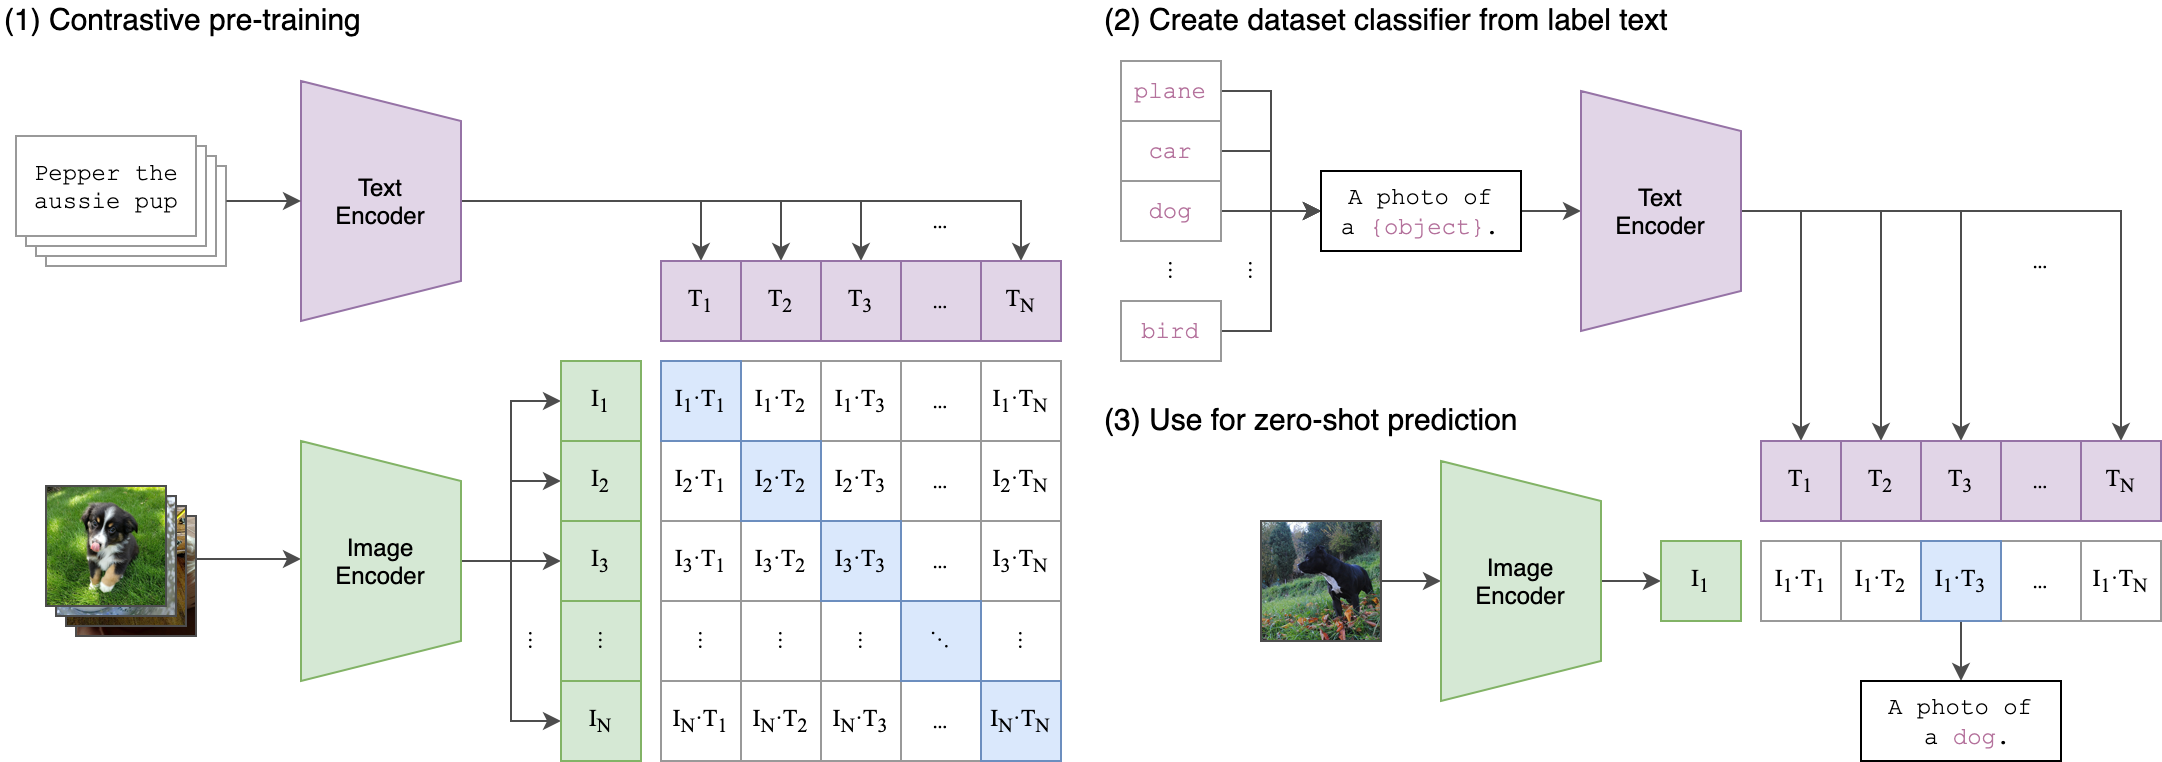
\includegraphics[width=0.95\textwidth]{CLIP.png}
  \caption{on the left an overview of the pretaining objective, on the right the zero shot classification task}
  \label{fig:clip}
\end{figure*}

\section{CLIP} %maybe not the first section, text in progress
The CLIP \cite{radford2021learning} architecutre uses contrastive loss to learn a common embedding space for image, text pairs.
It's based on consine similarity and can be used with a variety of text encoder as well as image encoders.
Figure \ref*{fig:clip} details the main task for CLIP, zero shot image calssifcation.
A single pretrained model can outperform task specific and finetuned models on various benchmarks.


\subsection{Applications} %I will look for a reference on those saliency maps -found none
CLIP is the backbone for many text to image generation models such as DALL-E 2 \cite{ramesh2022hierarchical} ("unclip").
The similary of a generated image to the provided input prompt gives the model feedback to learn from.
On the academic side, a shared task like Visual Word Sense Disambiguation \cite{raganato-etal-2023-semeval} has been approached by CLIP and drivates by most submissions.

\subsection{following research} %better title needed
Building upon the idea of CLIP is models like BLIP\cite{li2022blip} which focus to sovle visual question answering by using a generative text decoder.

% \clearpage % trying to fit it all on the two pages.
\bibliography{acl2020}
\bibliographystyle{acl_natbib}

\appendix
\end{document}
